\documentclass{article}
\usepackage[utf8]{inputenc}
\usepackage{subcaption}
\usepackage{graphicx}
\usepackage[margin=2.5cm]{geometry}
\usepackage{array}
\usepackage{wrapfig}
\usepackage{multirow}
\usepackage{tabularx}
\usepackage{amsmath}
\usepackage{wrapfig}
\usepackage{mathtools}
\usepackage{gensymb}
\usepackage[table]{xcolor}
\usepackage{xcolor,colortbl}
\usepackage{multirow}
\usepackage{polski}
\title{Sprawozdanie 4\\ Ćwiczenie 57c}
\author{Jan Bronicki \\
Nr indeksu: 249011\\
Marcin Radke\\
Nr indeksu: 241554}
\date{}
\begin{document}

\maketitle
%------------------------------------------------------------------
% WSTEP TEORETYCZNY
\section{Wstęp Teoretyczny}
\par Celem ćwiczenia jest zbadanie efektu Halla. Zmierzymy $U_{H}$ w zależności od $\alpha$, gdzie $U_{H}$ jest napięciem jakie powstaje w skutek efektu Halla kiedy kręcimy hallotronem, a $\alpha$ jest kątem o, który przekręciliśmy go. Narysujemy zatem wykresy, dla $U_{H}(\alpha)$ oraz $U_{H}(B_{n})$. Następnie na podstawie wykresów $U_{H}(B_{n})$ i $U_{H}(I_{s})$, które powinny przypominać swoimi charakterystykami wykresy liniowe wyznaczymy wspołczynnik $\gamma$, gdzie $U_{H}=\gamma I_{s}$. Następnie $\gamma$ posłuży nam do obliczenia koncentracji ładunków $n=\frac{1}{\gamma e d}$, gdzie $e$ - ładunek, $d$ - gęstość.

\begin{figure}[h]
    \centering
    \caption{Schemat Hallotronu}
    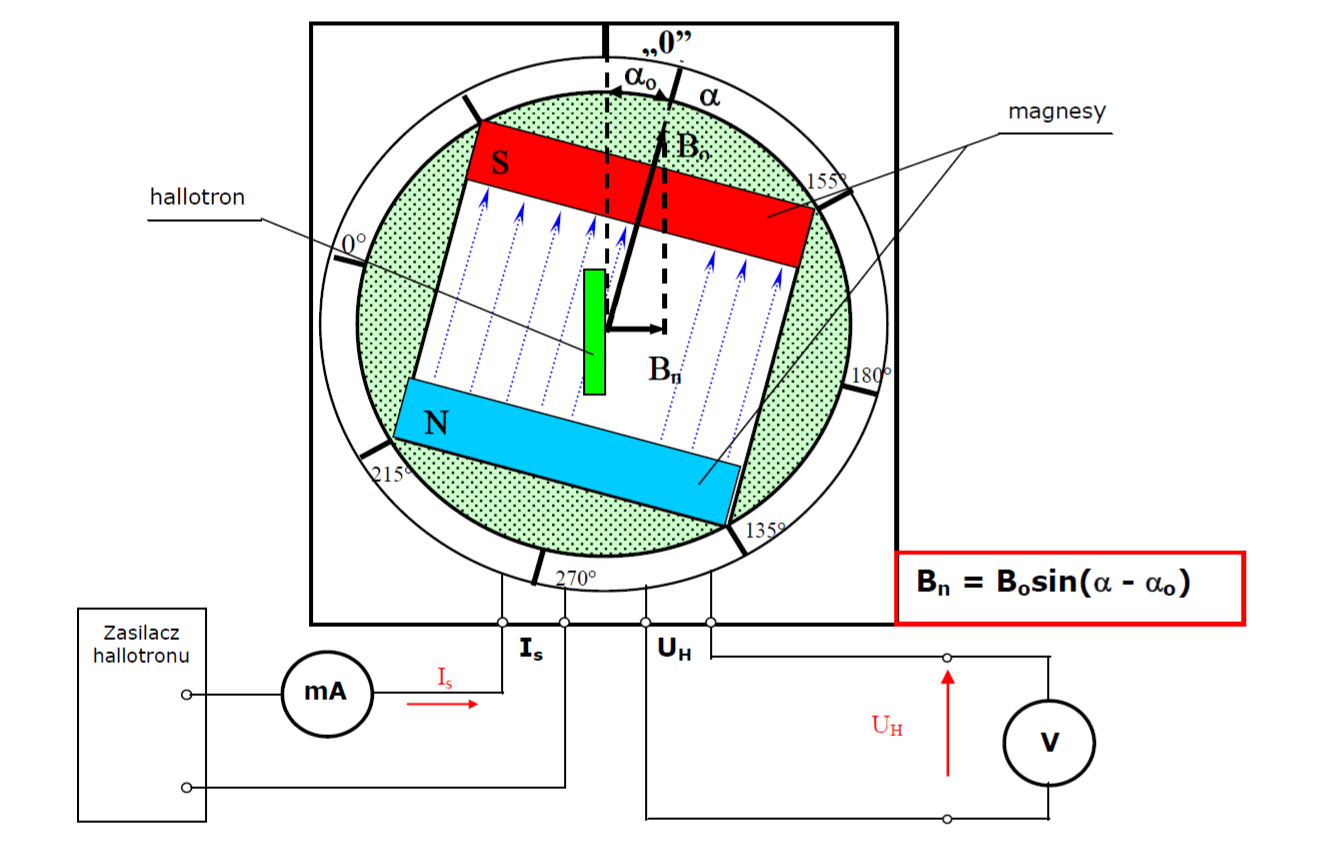
\includegraphics[width=8cm]{schemat_hallotronu.png}
    \label{fig:rys1}
\end{figure}

W naszym eksperymencie wykorzystamy następujące przyrządy:
\begin{itemize}
    \item Hallotron umieszczony w polu magnetycznym wytworzonym przez Magnesy trwałe. Magnesy zamocowane są         tak, by możliwy był pomiar zmian orientacji pola magnetycznego względem płaszczyzny hallotronu
    \item Zasilacz hallotronu
    \item Miliamperomierz do pomiaru natężenia prądu sterującego $I_{s}$
    \item Woltomierz do pomiaru napięcia Hall'a $U_{H}$
    \item Przewody elektryczne
\end{itemize}
% WSTEP TEORETYCZNY
%------------------------------------------------------------------
\newpage
%------------------------------------------------------------------
% OPRACOWANIE WYNIKOW
\section{Opracowanie wyników}

% Wykres UH(alfa)
Sporządziliśmy wykres $U_{H}(\alpha)$:
\begin{figure}[h]
    \centering
    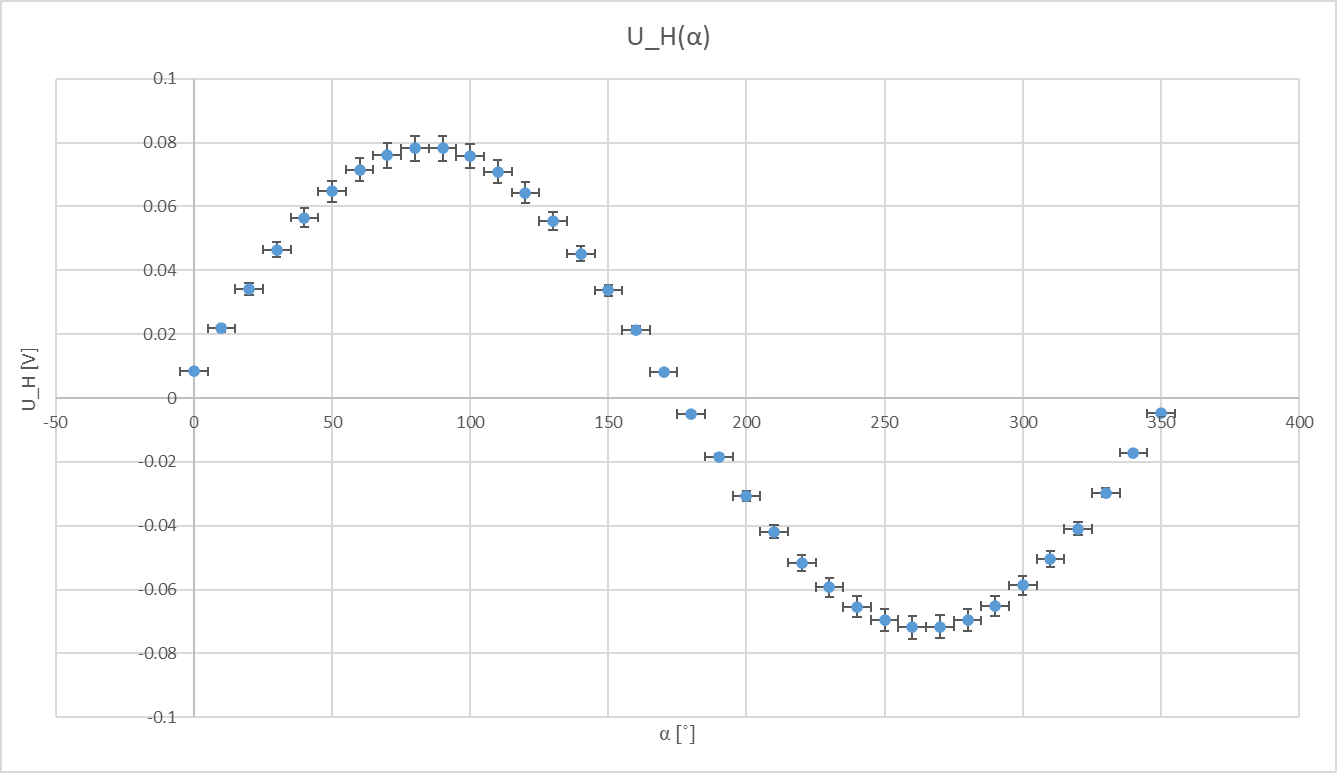
\includegraphics{U_H_od_ALFA.png}
    \caption{Wykres napięcia hallotronu od kąta}
    \label{fig:rys2}
\end{figure}

% Przykladowe niepewnosci UH(alfa)
\begin{figure}[h]
    Oto przykładowe niepewności:
    \begin{itemize}
        \item Niepewność kąta $\alpha$ założyliśmy jako stałą wynoszącą $5^{\circ}$ (w radianach $\approx 0.0873$)
        \item $u(U_{H})=\pm(0.05\cdot rdg +3\cdot dgt)=\pm(0.05\cdot0.00832
     +3\cdot 0.00001)\approx\pm0.0004 \ V$
    \end{itemize}
    Odczytana z wykresu wartość $\alpha_{0} \approx 175^{\circ}$.
\end{figure}

% Wykres UH(Bn)
Na podstawie wzoru $B_{n}=B_{0}sin(\alpha-\alpha_{0})$ został narysowany wykres \ref{fig: Wykres 3} opisujący $U_{H}(B_{n})$. Jako wartość $B_{0}$ zgodnie z instrukcją przyjęte zostało $0.5$, a błąd $B_{0}=\pm0.05 \ T$.\\
\begin{figure}[h]
Przykładowe obliczenia $B_{n}$ oraz jej niepewności:
    \begin{itemize}
        \item $B_{n}=B_{0}sin(\alpha-\alpha_{0})=0.5\cdot sin(0^{\circ}-175^{\circ})\approx -0.04358 \ T$
        \item $u(B_{n})=\sqrt{(B_{0}^{2}\cdot cos^{2}(\alpha-175^{\circ})\cdot u^{2}(\alpha)+sin^{2}(\alpha-175^{\circ})\cdot u^{2}(B_{0})}=\\=\sqrt{(0.5^{2}\cdot cos^{2}(0^{\circ}-175^{\circ})\cdot 0.0873^{2}+sin^{2}(0^{\circ}-175^{\circ})\cdot 0.05^{2}}\approx \pm0.00578 \ T$
        \item Niepewność $u(\alpha) = \pm5^{\circ}$ została wyrażona w radianach i wynosi około $\pm0.0873 \ \left[rad\right]$
    \end{itemize}{}
\end{figure}


\begin{figure}[h]
    \centering
    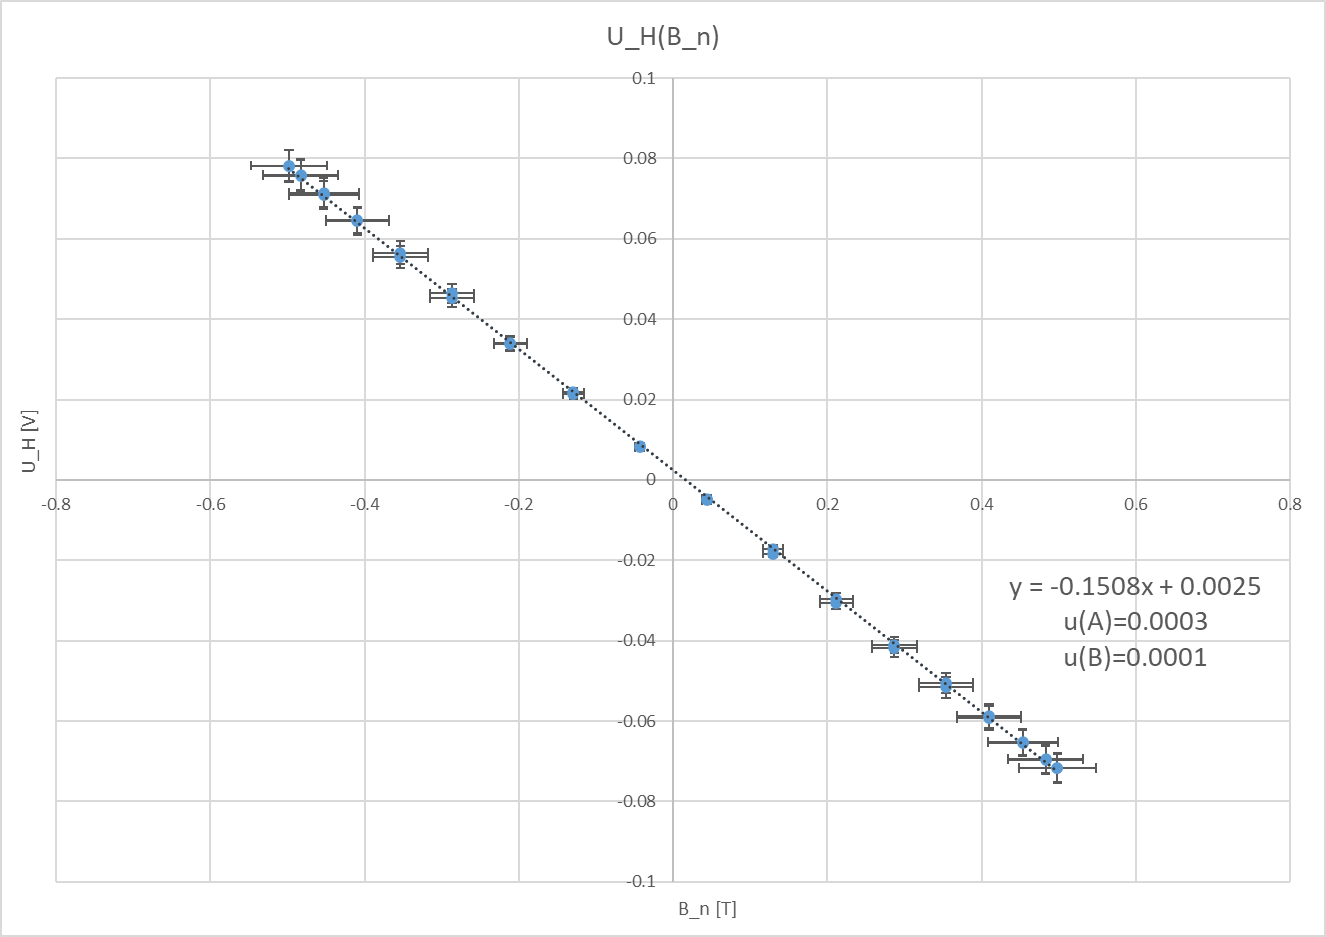
\includegraphics{U_H_od_B_n.png}
    \caption{Wykres napięcia hallotronu $U_{H}$ od indukcji magnetycznej $B_{n}$ }
    \label{fig: Wykres 3}
\end{figure}{}
Dzięki wykresowi \ref{fig: Wykres 3} uzyskujemy jego linię regresji $y=Ax+B$, gdzie $|A|=\gamma I_{s}$ z czego otrzymujemy, że $\gamma=\cfrac{|A|}{I_{s}}$, dla rozróżnienia tutaj otrzymanego współczynnika $\gamma$ dopasujemy mu indeks "s" otrzymując $\gamma_{s}=\frac{|A|}{I_{s}}$.
\begin{center}
$
    y=-0.1508x+0.0025\\
    u(A)\approx\pm0.0003, u(B)\approx\pm0.0001
$
\end{center}{}
\newpage
Na tej podstawie możemy wyliczyć $\gamma_{s}$.
\begin{center}
    \vspace{2.5ex}
    $\gamma_{s}=\frac{|A|}{I_{s}}=\frac{0.1508}{0.005}\approx30.16$\\
    \vspace{2.5ex}
    $u(A)=\pm0.0003$\\
    \vspace{2.5ex}
    $u(I)=\frac{Klasa\cdot Zakres}{100\cdot \sqrt{3}}=\frac{0.5\cdot0.0075}{100\cdot \sqrt{3}}\approx\pm0.0002 \ A$\\
    \vspace{2.5ex}
    $u(\gamma_{s})=\sqrt{\sum^{k}_{j=1}\left(\frac{\partial f}{\partial x_{j}}\right)^{2}\cdot u^{2}(x_{j})}=\sqrt{u^{2}(A)\cdot\left(\frac{1}{I_{s}}\right)^{2}+u^{2}(I_{s})\cdot(\frac{A}{I_{s}^{2}})^{2}}=$\\
    \vspace{2.5ex}
    $=\sqrt{0.0003^{2}\cdot\left(\frac{1}{0.005}\right)^{2}+0.0002^{2}\cdot(\frac{0.1508}{0.005^{2}})^{2}}  \approx\pm1.21$\\
    \vspace{2.5ex}
\end{center}
W związku z sinsoidą zawartą we wzorze na $B_{n}$ niepewność $B_{n}$ waha się oraz w pewnych momentach (widzianych na skrajnych wartościach indukcji) owe niepewności osiągają dość duże wartości. Co za tym idzie $\gamma_{s}$, która jest na podstawie wyliczonych $B_{n}$ obliczana również jest opatrzona sporą wartością niepewności.\\

\newpage

\par Następnie ponownie spróbujemy wyliczyć współczynnik $\gamma$ tym razem na podstawie pomiarów napięcia $U_{H}$ od natężenia $I_{s}$ (które tym razem nie jest stałe i jest przedmiotem naszych pomiarów). Jak widać na otrzymanym wykresie \ref{fig:Wykres 4} zależność, którą utrzymaliśmy jest liniowa, a w tym przypadku mając $y=Ax+B$ współczynnik $A$ będzie się równał $A=\gamma B$. Ponownie, dla rozróżnienia wspołczynnikowi $\gamma$ tutaj otrzymanemu nadamy indeks, dla jego rozróżnienia ("h"). Tak więc otrzymujemy taką zależność $\gamma_{h}=\frac{|A|}{B}$. W tych pomiarach indukcja $B$ jest taka, że $B=const.$.



\begin{figure}
    \centering
    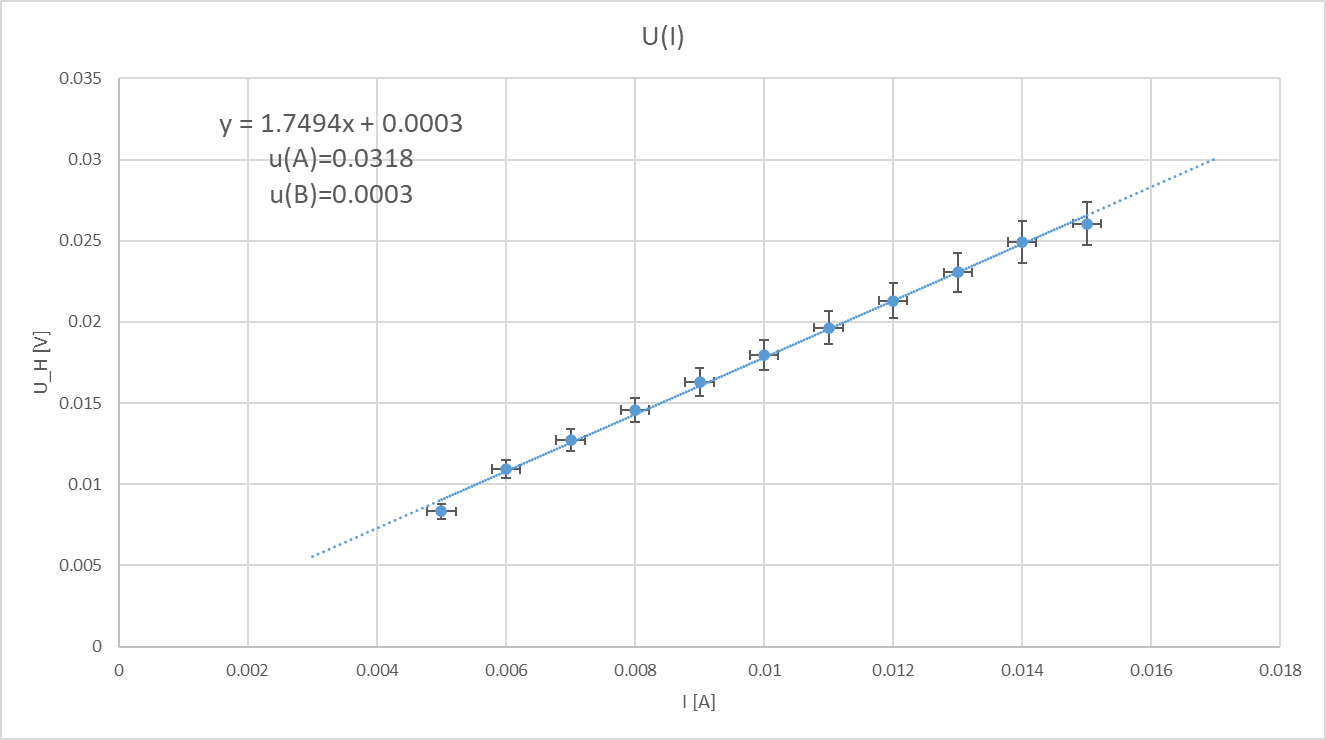
\includegraphics{U_H_od_I.png}
    \caption{Wykres napięcia $U_{H}$ od natężenia $I_{s}$}
    \label{fig:Wykres 4}
\end{figure}
% OPRACOWANIE WYNIKOW
%------------------------------------------------------------------



\end{document}
